% !TeX spellcheck = en_GB

\documentclass[10pt,xcolor=pdftex,dvipsnames,table]{beamer}

\usetheme{Boadilla}

\usepackage{lmodern}
\usepackage[T1]{fontenc}     % caracteres accentues
\usepackage[utf8]{inputenc}  %  encodage unicode des sources .tex
\usepackage{amsmath,amssymb,amsbsy,dsfont}

% pour \mybox...
\usepackage{xcolor}
\setlength{\fboxrule}{0.1pt}
\newcommand{\mybox}[2]{\fcolorbox{#1}{white}{$\displaystyle#2$}}


\title{FEM for 2D Linear Elasticity}
\author{ MATH-0471 }
%\institute{University of Li\`ege}
\date{\today}

%\AtBeginSection[]
%{
%	\begin{frame}
%		\frametitle{Outline}
%		\tableofcontents[currentsection]
%	\end{frame}
%}


\begin{document}

\frame{\titlepage}

%\section*{Outline}

%\begin{frame}
%	\frametitle{Outline}
%	\tableofcontents
%\end{frame}

% ---------------------------------------------------------------------------------------
%\section{ FEM for 2D Linear Elasticity  }
% ---------------------------------------------------------------------------------------
\begin{frame}
	\frametitle{ FEM for 2D Linear Elasticity }
	\framesubtitle{ Summary of equations }
	
	\textbf{Mechanical equilibrium} in $\Omega$:
	
	\begin{equation*}
		\left\{
		\begin{aligned}
		 \boldsymbol{\nabla}\cdot\boldsymbol{\sigma} + \rho\boldsymbol{b} &= 0
		\qquad &&\text{ (translation) } \\
		 \boldsymbol{\sigma} &= \boldsymbol{\sigma}^T &&\text{ (rotation) }
		\end{aligned}
	\right.
	\end{equation*}
	
	where $\boldsymbol{\sigma}$ is the Cauchy stress tensor, $\rho$ is the density and $\boldsymbol{b}$ represents the mechanical volumic forces.	
	
	\vspace{\stretch{1}}
	
	
and the \textbf{boundary conditions} on $\Gamma$, the boundary of $\Omega$:

\begin{equation*}
	\left\{
	\begin{aligned}
		&  \boldsymbol{u} = \bar{\boldsymbol{u}}     & \qquad \text { on } \Gamma_{\bar{\boldsymbol{u}}} & \qquad \text{ : prescribed displacement (Dirichlet)} \\
		&  \boldsymbol{\sigma}\cdot\boldsymbol{n}  = \bar{\boldsymbol{t}}     & \text { on } \Gamma_{\bar{\boldsymbol{t}}} & \qquad \text{ : prescribed surface traction (Neumann)} \\
	\end{aligned}
	\right.    
\end{equation*}	
where $\boldsymbol{u}$ is the displacement, $\boldsymbol{n}$ is the outward unit normal to the boundary, $\Gamma_{\bar{\boldsymbol{u}}} \cup \Gamma_{\bar{\boldsymbol{t}}} = \Gamma$ and $\Gamma_{\bar{\boldsymbol{u}}} \cap \Gamma_{\bar{\boldsymbol{t}}} = \emptyset$


\end{frame}

\begin{frame}
	\frametitle{ FEM for 2D Linear Elasticity }
	\framesubtitle{ Summary of equations }

	\textbf{Strain-displacement relationship} (infinitesimal strains):
	\begin{equation*}
		\boldsymbol{\varepsilon} 
		= \tfrac{1}{2} \left( \boldsymbol{\nabla}\boldsymbol{u} + (\boldsymbol{\nabla}\boldsymbol{u})^T \right) 
	\end{equation*}
	where small strains and small displacements are assumed.

	\vspace{\stretch{1}}

	\textbf{Constitutive law} (Hooke's law):
	\begin{equation*}
		\boldsymbol{\sigma} = \mathbb{H}:\boldsymbol{\varepsilon}
	\end{equation*}
	with the 4$^{th}$ order tensor
	\begin{equation*}
		\mathbb{H}_{ijkl} = \frac{E}{2(1+\nu)} \delta_{ik}\delta_{jl}
		+ \frac{\nu\,E}{(1+\nu)(1-2\nu)}\delta_{ij}\delta_{kl}
		\quad\text{ with }
		\left\{
		\begin{aligned}
			&E : \text{Young's modulus} \\
			&\nu : \text{Poisson's ratio} \\
		\end{aligned}
		\right.
	\end{equation*}	
	for an isotropic material.
\end{frame}




\begin{frame}
	\frametitle{ FEM for 2D Linear Elasticity }
	\framesubtitle{ Weak formulation }
	
	A \textbf{weak formulation} is obtained by multiplying the PDE by a function $\boldsymbol{w}(\boldsymbol{x})$ and by integrating over $\Omega$:
	
	\begin{equation*}
		\int_{\Omega} \boldsymbol{w}\cdot \left(\boldsymbol{\nabla}\cdot\boldsymbol{\sigma}\right)\, dV 
		+ \int_{\Omega} \rho \boldsymbol{w}\cdot \boldsymbol{b}\, dV = 0
	\end{equation*}	

	\vspace{\stretch{1}}

	The first term of the left-hand side can be integrated by parts:
	\begin{equation*}
	\int_{\Omega} \boldsymbol{w}\cdot \left(\boldsymbol{\nabla}\cdot\boldsymbol{\sigma}\right)\, dV 
	= \int_{\Gamma_{\bar{\boldsymbol{u}}}} \boldsymbol{w}\cdot \boldsymbol{\sigma} \cdot \boldsymbol{n}\, dS
	+ \int_{\Gamma_{\bar{\boldsymbol{t}}}} \boldsymbol{w}\cdot \underbrace{\boldsymbol{\sigma} \cdot \boldsymbol{n}}_{\boldsymbol{\bar{t}}}\, dS
	- \int_{\Omega} \boldsymbol{\nabla}\boldsymbol{w} : \boldsymbol{\sigma}\, dV
	\end{equation*}	
	
	The integral on $\Gamma_{\bar{u}}$ can disappear if we choose test functions $\boldsymbol{w}(\boldsymbol{x})$ that vanish on this boundary.
\end{frame}


\begin{frame}
	\frametitle{ FEM for 2D Linear Elasticity }
	\framesubtitle{ Weak formulation }
	
	Moreover, since $\boldsymbol{\sigma} = \boldsymbol{\sigma}^T$, we can write
	
	\begin{equation*}
		\boldsymbol{\nabla}\boldsymbol{w} : \boldsymbol{\sigma} = \underbrace{\tfrac{1}{2} \left( \boldsymbol{\nabla}\boldsymbol{w} + (\boldsymbol{\nabla}\boldsymbol{w})^T \right)}_{\text{similar to } \boldsymbol{\varepsilon}(\boldsymbol{u})} : \boldsymbol{\sigma}
	\end{equation*}	
	
	
	\vspace{\stretch{1}}	
	
	The weak formulation becomes\footnote{This is also called ``the principle of virtual work''. \\
		Notations in \cite{ponthot2020}: $\boldsymbol{w} \leftrightarrow \boldsymbol{\delta u}$ and $\boldsymbol{\delta \varepsilon} \leftrightarrow \tfrac{1}{2} \left( \boldsymbol{\nabla}\boldsymbol{w} + (\boldsymbol{\nabla}\boldsymbol{w})^T \right)$) \\
		and $\boldsymbol{u}+\boldsymbol{\delta u}=\boldsymbol{\bar{u}}$ on $\Gamma_{\bar{u}}$ (``kinematically admissible virtual displacement'').\\}:
	
	\begin{block}{Weak formulation}
		Find $\boldsymbol{u}$ with $\boldsymbol{u} = \bar{\boldsymbol{u}}$ on $\Gamma_{\bar{u}}$   such that
		\begin{equation*}
			\int_{\Gamma_{\bar{\boldsymbol{t}}}} \boldsymbol{w}\cdot \boldsymbol{\bar{t}}\, dS
			- \int_{\Omega} \tfrac{1}{2} \left( \boldsymbol{\nabla}\boldsymbol{w} + (\boldsymbol{\nabla}\boldsymbol{w})^T \right) : \boldsymbol{\sigma}\, dV		
			+ \int_{\Omega} \rho\boldsymbol{w} \cdot \boldsymbol{b}\, dV = 0
		\end{equation*}	
		for all test functions $\boldsymbol{w}$ which are 0 on $\Gamma_{\bar{u}}$.
	\end{block}
	
\end{frame}


\begin{frame}
	\frametitle{ FEM for 2D Linear Elasticity }
	\framesubtitle{ Spatial discretization - Finite Element approximation }
	
	The discretization procedure is similar to the one followed for the Laplace/Poisson equation in MATH0024, except that the unknown field $\boldsymbol{u}(\boldsymbol{x}, t)$ is now a vector instead of a scalar.	The equations are detailed here for the 2D case.	
	\vspace{\stretch{1}}
	
	Using Cartesian coordinates, each component of $\boldsymbol{u}(\boldsymbol{x}, t)$ and $\boldsymbol{w}(\boldsymbol{x})$ are approximated using well-chosen shape functions $N^k$:
	\begin{equation*}
		\left\{
		\begin{aligned}
			&u_1(\boldsymbol{x}, t) = \sum_k N^k(\boldsymbol{x})\,u_1^k(t) \\
			&u_2(\boldsymbol{x}, t) = \sum_k N^k(\boldsymbol{x})\,u_2^k(t) \\
		\end{aligned}
		\right.
		\quad
		\text{ and }
		\left\{
		\begin{aligned}
			&w_1(\boldsymbol{x}) = \sum_k N^k(\boldsymbol{x})\,w_1^k \\
			&w_2(\boldsymbol{x}) = \sum_k N^k(\boldsymbol{x})\,w_2^k \\
		\end{aligned}
		\right.		
	\end{equation*}	
	where $u_i^k$ is the $i^{\text{th}}$ coordinate of node $k$ (also called ``degree of freedom'').	
\end{frame}


\begin{frame}
	\frametitle{ FEM for 2D Linear Elasticity }
	\framesubtitle{ Spatial discretization - Finite Element approximation }
	
	In matrix form (assuming a mesh of $n$ nodes in a 2D space):
	\begin{equation*}
		\boldsymbol{u}(\boldsymbol{x},t) = \mathbf{N}(\boldsymbol{x})\,\boldsymbol{d}(t)
	\end{equation*}	
	with
	\begin{equation*}
		\mathbf{N}(\boldsymbol{x}) = 
		\begin{bmatrix}
			N_1 & 0      & N_2 & 0      & \dots & N_n & 0 \\
			0   & N_1    & 0   & N_2    & \dots & 0 & N_n \\
		\end{bmatrix}
	\end{equation*}		
	\begin{equation*}
		\boldsymbol{d}^T = 
		\begin{bmatrix}
			u_1^1 & u_2^1  & u_1^2 & u_2^2 &  \dots & u_1^n & u_2^n
		\end{bmatrix}
	\end{equation*}
	
	\vspace{\stretch{1}}
	
	Similarly, for the test functions:
	\begin{equation*}
		\boldsymbol{w}(\boldsymbol{x}) = \mathbf{N}(\boldsymbol{x})\,\boldsymbol{h}
	\end{equation*}	
\end{frame}



\begin{frame}
	\frametitle{ FEM for 2D Linear Elasticity }
	\framesubtitle{ Isoparametric Finite Elements }
	
	
	\centerline{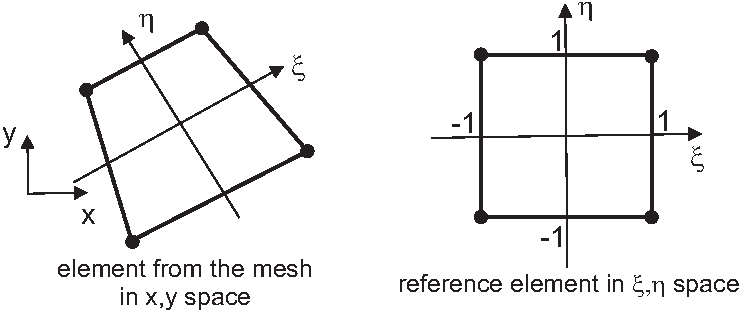
\includegraphics[width=0.7\textwidth]{fig_isoparametric}}
	
	\vspace{\stretch{1}}
	
	\textbf{Isoparametric finite elements} ($m$ nodes) are a classical choice. Their geometry is interpolated with the same shape functions\footnote{$N^k$: superscript $k$ is related nodes where $N^k=1$}
	as the unknown field $\boldsymbol{u}(\boldsymbol{x}, t)$ and the test functions $\boldsymbol{w}(\boldsymbol{x})$.
	\begin{equation*}
		\boldsymbol{x}(\boldsymbol{\xi}) = \sum_{k=1}^m N^k(\boldsymbol{\xi})\,\boldsymbol{x}^k
	\end{equation*}	
	where $\boldsymbol{\xi}$ are reduced coordinates (usually $\xi_i\in[-1,1]$)
\end{frame}



\begin{frame}
	\frametitle{ FEM for 2D Linear Elasticity }
	\framesubtitle{ 3D Hooke's law (matrix form) }
	
	\textbf{Voigt's notation}: in a practical implementation, $4^{\text{th}}$ and $2^{\text{nd}}$-order tensors are replaced by matrices and vectors respectively.
	\begin{equation*}
		\begin{bmatrix}
			\sigma_{11} \\
			\sigma_{22} \\
			\sigma_{33} \\
			\sigma_{12} \\
			\sigma_{13} \\
			\sigma_{23} \\	
		\end{bmatrix}
		= \frac{E}{(1+\nu)(1-2\nu)}
		\begin{bmatrix}
			1-\nu & \nu & \nu & 0 & 0 & 0 \\
			\nu & 1-\nu &  \nu & 0 & 0 & 0 \\
			\nu & \nu & 1-\nu &  0 & 0 & 0 \\
			0 &0 & 0 & \frac{1-2\nu}{2} & 0 & 0 \\
			0 &0 & 0 & 0 &\frac{1-2\nu}{2}  & 0 \\
			0 &0 & 0  & 0 & 0 & \frac{1-2\nu}{2} \\
		\end{bmatrix}
		\begin{bmatrix}
			\varepsilon_{11} \\
			\varepsilon_{22} \\
			\varepsilon_{33} \\
			2\varepsilon_{12} \\
			2\varepsilon_{13} \\
			2\varepsilon_{23} \\	
		\end{bmatrix}			
	\end{equation*}	
	such that
	\begin{equation*}
		\boldsymbol{\varepsilon}:\boldsymbol{\sigma} = \boldsymbol{\varepsilon}^v\cdot \boldsymbol{\sigma}^v
	\end{equation*}	
	
	Hooke's law becomes:
	\begin{equation*}
		\boldsymbol{\sigma}^v = \mathbf{H}\,\boldsymbol{\varepsilon}^v
	\end{equation*}		

	\vspace{\stretch{1}}
		
	Remark: $\boldsymbol{\varepsilon}^v$ involves ${\color{red}2\times}\varepsilon_{ij}$ = $\gamma_{ij}$ (shear strain/angle) for $i\neq j$.

\end{frame}



\begin{frame}
	\frametitle{ FEM for 2D Linear Elasticity }
	\framesubtitle{ 2D Hooke's law (matrix form) }
	
	A very common 2D assumption is the \textbf{plane-stress hypothesis} which is valid for thin structures  ($\sigma_{33}=\sigma_{13}=\sigma_{23}=0$):
	
	\begin{equation*}	
		\begin{bmatrix}
			\varepsilon_{11} \\
			\varepsilon_{22} \\
			\varepsilon_{33} \\
			2\varepsilon_{12} \\
			2\varepsilon_{13} \\
			2\varepsilon_{23} \\	
		\end{bmatrix}
	= \underbrace{\frac{1}{E}
	\begin{bmatrix}
		1 & -\nu & -\nu & 0 & 0 & 0 \\
		-\nu & 1 &  -\nu & 0 & 0 & 0 \\
		-\nu & -\nu & 1 &  0 & 0 & 0 \\
		0 &0 & 0 & \frac{1+\nu}{2} & 0 & 0 \\
		0 &0 & 0 & 0 &\frac{1+\nu}{2}  & 0 \\
		0 &0 & 0  & 0 & 0 & \frac{1+\nu}{2} \\
	\end{bmatrix}}_{\boldsymbol{H}^{-1}}		
	\begin{bmatrix}
		\sigma_{11} \\
		\sigma_{22} \\
		\color{red}0 \\
		\sigma_{12} \\
		\color{red}0 \\
		\color{red}0 \\	
	\end{bmatrix}				
	\end{equation*}	

	\vspace{\stretch{1}}
	
	The 2D Hooke's law is obtained by inverting this relationship:
	\begin{equation*}	
		\begin{bmatrix}
			\sigma_{11} \\
			\sigma_{22} \\
			\sigma_{12} \\
		\end{bmatrix}	
		= \underbrace{\frac{E}{1-\nu^2}
		\begin{bmatrix}
			1 & \nu &  0 \\
			\nu & 1 &  0 \\
			0  & 0 & \frac{1-\nu}{2}  \\
		\end{bmatrix}	}_{\boldsymbol{H}_{2D}}	
		\begin{bmatrix}
			\varepsilon_{11} \\
			\varepsilon_{22} \\
			2\varepsilon_{12} \\
		\end{bmatrix}			
	\end{equation*}		
	This $3\times 3$ matrix is used as $\boldsymbol{H}$ in the following equations.

\end{frame}


\begin{frame}
	\frametitle{ FEM for 2D Linear Elasticity }
	\framesubtitle{ Strain-displacement relationship }
	
	Using Voigt's notation, the strain-displacement relationship becomes:
	
	\begin{equation*}
		\begin{bmatrix}
			\varepsilon_{11} \\
			\varepsilon_{22} \\
			2\varepsilon_{12} \\
		\end{bmatrix}
		=
		\begin{bmatrix}
			\frac{\partial}{\partial x_1} & 0  \\
			0 &\frac{\partial}{\partial x_2}  \\
			\frac{\partial}{\partial x_2} & \frac{\partial}{\partial x_1}  \\
		\end{bmatrix}
		\begin{bmatrix}
			u_1 \\	
			u_2 \\
		\end{bmatrix}						
	\end{equation*}	
	
	or, symbolically
	\begin{equation*}
		\boldsymbol{\varepsilon}^v = \boldsymbol{\partial}\,\boldsymbol{u}
	\end{equation*}		
	
	\vspace{\stretch{1}}	
	
	Remarks:
	\begin{itemize}
	\item $\varepsilon_{33}$ does not appear in the 2D equations. However, it can be computed, if needed, from the stresses:
	\begin{equation*}	
	 	\varepsilon_{33}=-\frac{\nu}{E}\left(\sigma_{11}+\sigma_{22}\right) 
	\end{equation*}	
	\item Strains (and stresses) are discontinuous across finite elements boundaries unless $\boldsymbol{u}(\boldsymbol{x})$ is $C^1$, which is almost never the case in practise.
	\end{itemize}
\end{frame}



\begin{frame}
	\frametitle{ FEM for 2D Linear Elasticity }
	\framesubtitle{ Strains/stresses as a function of the unknowns}
	
	Computation of \textbf{strains} from the nodal displacements $\boldsymbol{d}$:
	\begin{equation*}
		\boldsymbol{\varepsilon}^v = \boldsymbol{\partial}\,\boldsymbol{u} = 	\boldsymbol{\partial}\,\mathbf{N}\,\boldsymbol{d} = \mathbf{B}\,\boldsymbol{d}
	\end{equation*}		
	with
	\begin{equation*}
	\mathbf{B} =
		\begin{bmatrix}
			\frac{\partial}{\partial x_1} & 0  \\
			0 &\frac{\partial}{\partial x_2}  \\
			\frac{\partial}{\partial x_2} & \frac{\partial}{\partial x_1}   \\
		\end{bmatrix}
		\begin{bmatrix}
			N^1 & 0      &  \dots & N^m & 0 \\
			0   & N^1    &  \dots & 0 & N^m  \\
		\end{bmatrix}	
	\end{equation*}
	
	
	\vspace{\stretch{1}}
		
	The \textbf{stresses} can also be obtained from the nodal displacement $\boldsymbol{d}$: 

	\begin{equation*}
		\boldsymbol{\sigma}^v = \mathbf{H}\,\mathbf{B}\,\boldsymbol{d}
	\end{equation*}		
	
\end{frame}


\begin{frame}
	\frametitle{ FEM for 2D Linear Elasticity }
	\framesubtitle{ Discretized weak formulation }
	
	Back to the \textbf{weak formulation}
	\begin{equation*}
		\int_{\Gamma_{\bar{\boldsymbol{t}}}} \boldsymbol{w}\cdot \boldsymbol{\bar{t}}\, dS
		- \int_{\Omega} 
		\underbrace{\frac{1}{2} \left( \boldsymbol{\nabla}\boldsymbol{w} + (\boldsymbol{\nabla}\boldsymbol{w})^T \right) 
		: \boldsymbol{\sigma}}_{(\mathbf{B}\boldsymbol{h})\cdot\boldsymbol{\sigma}^v }\, dV		
		+ \int_{\Omega} \rho \boldsymbol{w} \cdot \boldsymbol{b}\, dV = 0
	\end{equation*}	
	
	
	\vspace{\stretch{1}}
	
	Replacing $\boldsymbol{w}=\mathbf{N}\boldsymbol{h}$ and $\boldsymbol{u}=\mathbf{N}\boldsymbol{d}$ and $\boldsymbol{\sigma}^v = \mathbf{H}\,\mathbf{B}\,\boldsymbol{d}$	
	
	
	\begin{equation*}
			\boldsymbol{h}^T \left( \int_{\Gamma_{\bar{\boldsymbol{t}}}} \mathbf{N}^T\boldsymbol{\bar{t}}\, dS \right)  - \boldsymbol{h}^T \left(\int_{\Omega}\mathbf{B}^T\mathbf{H}\mathbf{B} \, dV \right) \boldsymbol{d}
			+ \boldsymbol{h}^T \left( \int_{\Omega} \rho\mathbf{N}^T\boldsymbol{b}\, dV \right) = 0
	\end{equation*}		
	
	This relationship should be satisfied for any $\boldsymbol{h}$.
	
\end{frame}




\begin{frame}
	\frametitle{ FEM for 2D Linear Elasticity }
	\framesubtitle{ Discretized FE equations }
	
	This leads to the system of discretized equations:
	\begin{equation*}
		\underbrace{\left(\int_{\Omega}\mathbf{B}^T\mathbf{H}\mathbf{B} \, dV \right)}_{\mathbf{K}} \boldsymbol{d}		
		= 
		\underbrace{\left( \int_{\Gamma_{\bar{\boldsymbol{t}}}} \mathbf{N}^T\boldsymbol{\bar{t}}\, dS \right)
		+  \left( \int_{\Omega} \rho\,\mathbf{N}^T\boldsymbol{b}\, dV \right)}_{\boldsymbol{f}}
	\end{equation*}		
	
		\vspace{\stretch{1}}
		
	\begin{block}{Discretized equations}	
		\begin{equation*}
			\mathbf{K}\boldsymbol{d}=\boldsymbol{f}
		\end{equation*}	
	\end{block}


\end{frame}

\begin{frame}
	\frametitle{ FEM for 2D Linear Elasticity }
	\framesubtitle{ Finite Elements }

	\textbf{Assembly}:
	\begin{itemize} 
		\item 	The integrals involved in the calculation of $\mathbf{K}$ and $\boldsymbol{f}$ are expressed as a sum of integrals over each finite element. These elemental contributions are then assembled (summed) in a large and structural matrix and vector.
		\item $\mathbf{K}$ is a symmetric sparse matrix and this property should be exploited to reduce the required storage and to efficiently solve the linear system of equations.
	\end{itemize}
	
	\vspace{\stretch{1}}
	
	\textbf{Boundary conditions}:
	\begin{itemize} 
		\item The equations of the system corresponding to nodes where Dirichlet boundary conditions are prescribed should be discarded and replaced by equations enforcing these conditions ($\boldsymbol{u}=\bar{\boldsymbol{u}}$) at these nodes.
		\item Homogeneous Dirichlet boundary conditions ($\boldsymbol{u}=0$) lead to remove the lines and columns of the matrices corresponding to the components of the displacement where these conditions are prescribed.
	\end{itemize}
\end{frame}


\begin{frame}
	\frametitle{ FEM for 2D Linear Elasticity }
	\framesubtitle{ Practical calculation of the elemental stiffness matrices }
	
	\begin{equation*}
		K_{ij} = \int_{\Omega} B_{ki}(\boldsymbol{x})\,H_{kl}\,B_{lj}(\boldsymbol{x}) \, dV
	\end{equation*}		
	\vspace{\stretch{1}}
	
	Isoparametric finite elements:
	\begin{equation*}
		K_{ij} = \int_{-1}^1\int_{-1}^1\int_{-1}^1 B_{ki}(\boldsymbol{\xi})\,H_{kl}\,B_{lj}(\boldsymbol{\xi})\, \underbrace{\det (\frac{\partial{\boldsymbol{x}} }{\partial\boldsymbol{\xi}})}_{\text{jacobian}}  \, d\boldsymbol{\xi}
	\end{equation*}		

	\vspace{\stretch{1}}
		
	\centerline{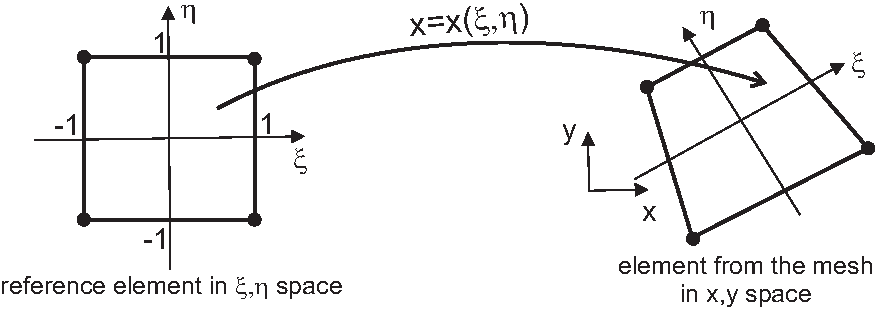
\includegraphics[width=0.8\textwidth]{fig_isoparametric2}}

\end{frame}


\begin{frame}
	\frametitle{ FEM for 2D Linear Elasticity }
	\framesubtitle{ Gauss quadrature }
	
	This integral is calculated using a Gauss quadrature: ($N^{\text{GP}}$ chosen $\rightarrow$  $\boldsymbol{\xi}^p$, $w_p$)
	
	\begin{equation*}
		K_{ij} \approx \sum_{p=1}^{N^{\text{GP}}} \underbrace{
			B_{ki}(\boldsymbol{\xi})\,H_{kl}\,B_{lj}(\boldsymbol{\xi})
			\det \mathbf{J}
		}_{\text{all the factors evaluated at } \boldsymbol{\xi}=\boldsymbol{\xi}^p} \,w_p
	\end{equation*}
	with $N^{\text{GP}}$, the number of Gauss points, $\boldsymbol{\xi}^p$ the positions and $w_p$, the weights.
	
	\vspace{\stretch{1}}
	\centerline{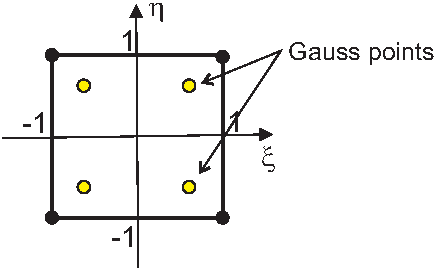
\includegraphics[width=0.4\textwidth]{fig_gauss}}

\end{frame}


\begin{frame}
	\frametitle{ FEM for 2D Linear Elasticity }
	\framesubtitle{ Jacobian of isoparametric elements at each Gauss points}
	
	\textbf{Jacobian matrix}\footnote{transposed in \cite{ponthot2020}}: let $\boldsymbol{x}=(x_1, x_2, x_3)$ and $\boldsymbol{\xi}=(\xi_1, \xi_2, \xi_3)$
	\begin{equation*}
		J_{ij} (\boldsymbol{\xi}) =\frac{\partial x_i}{\partial \xi_j} = \frac{\partial N^k (\boldsymbol{\xi})}{\partial \xi_j} x_i^k
	\end{equation*}	
	where $x_i^k$ is the $i^{\text{th}}$ coordinate of the $k^{\text{th}}$ node of the finite element.	
	
	\vspace{\stretch{1}}
	The Jacobian matrix and its determinant must be evaluated at each Gauss point ($\boldsymbol{\xi}=\boldsymbol{\xi}^p$) of each finite element. 
	
	\vspace{\stretch{1}}
	
	Note: the derivatives of the shape functions evaluated at the Gauss points $\frac{\partial N^k}{\partial \xi_j} (\boldsymbol{\xi}^p)$ are the same for all elements and can be computed once.	
	
\end{frame}




\begin{frame}
	\frametitle{ FEM for 2D Linear Elasticity }
	\framesubtitle{ Derivatives of the shape functions }
	
	\begin{equation*}
		\mathbf{B} =
		\begin{bmatrix}
			\frac{\partial}{\partial x_1} & 0  \\
			0 &\frac{\partial}{\partial x_2}  \\
			\frac{\partial}{\partial x_2} & \frac{\partial}{\partial x_1}   \\
		\end{bmatrix}
		\begin{bmatrix}
			N^1 & 0      &  \dots & N^m & 0 \\
			0   & N^1    &  \dots & 0 & N^m  \\
		\end{bmatrix}	
	\end{equation*}

	The matrix $\mathbf{B}$ contains the derivatives of the shape functions with respect to $\boldsymbol{x}$ which should be transformed into derivatives of the shape functions with respect to $\boldsymbol{\xi}$ using the Jacobian matrix:
	
	\begin{equation*}
		\frac{\partial}{\partial\xi_i} = \left( \frac{\partial x_j}{\partial \xi_i}  \right) \frac{\partial}{\partial x_j} = J_{ji} \frac{\partial}{\partial x_j} \qquad \Rightarrow \boldsymbol{\nabla}_{\color{red}\boldsymbol{x}} = \mathbf{J}^{-T} \boldsymbol{\nabla}_{\color{red}\boldsymbol{\xi}}
	\end{equation*}	
	
		\vspace{\stretch{1}}
		
	Thus, the derivative of $N^i$ with respect to $\boldsymbol{x}$ can be computed by this formula:
	
	\begin{equation*}
		\boldsymbol{\nabla}_{\boldsymbol{x}} N^i = \mathbf{J}^{-T} \boldsymbol{\nabla}_{\boldsymbol{\xi}} N^i
	\end{equation*}	
	
\end{frame}



%------------------------------------------------

\begin{frame}
	\frametitle{References}
	\footnotesize{
		\begin{thebibliography}{99} % Beamer does not support BibTeX so references must be inserted manually as below
			\bibitem[Ponthot, 2020]{ponthot2020} J.-P. Ponthot (2020)
			\newblock An Introduction to the Finite Element Method
			\newblock \emph{Lecture notes}, chapters 10 -- 11.
		\end{thebibliography}
	}
\end{frame}


\end{document}
